% Copyright 2026 Sreeram Anil
% SPDX-License-Identifier: CC-BY-4.0
% =============================================================================
%  Kalman-consensus pack filter — pack-level family
% =============================================================================
\chapter{Kalman-Consensus Pack Filter (Consensus)}
\label{ch:consensus}

\section*{At a glance}
\begin{tabular}{@{}l>{\raggedright\arraybackslash}p{0.76\textwidth}@{}}
Family & pack-level (common state + per-cell deviation), fully distributed \\
Header & \texttt{include/estkit/pack/consensus.hpp} \\
Registered name & \texttt{Consensus} \\
Structure & $N_c$ nodes on a graph $\mathcal{G}$ (ring by default, degree $d=2$) \\
Exchanged per node & $\hat{\vx}_j$ ($n_x$), $\bm{u}_j$ ($n_x$), $\bm{U}_j$ ($n_x(n_x{+}1)/2$) $=18$ numbers \\
Cost per step & \SI{6344}{\nano\second} for all $N_c=12$ nodes (\SI{529}{\nano\second} per node) \\
Memory & \SI{9224}{\byte} total (one shared model, $2(n_x+n_x^2)$ per node) \\
Primary references & \cite{olfatisaber2007dkf,olfatisaber2007consensus,olfatisaber2009kcf,olfatisaber2005embedded} \\
\end{tabular}

\section{Motivation and aerospace/BMS relevance}
The federated filter of Chapter~\ref{ch:federated} distributes the computation but keeps a
\emph{master}: every node talks to one central combiner. In a 400-cell flight battery built from
daisy-chained cell-monitor ASICs, that topology is not free --- the chain is physically a line, a
node only has wires to its immediate neighbours, and a star topology means routing every message
through the whole chain. The natural question is whether the nodes can reach the same answer by
talking \emph{only to their neighbours}.

That is the problem Olfati-Saber's distributed Kalman filter and its Kalman-consensus variant
(KCF) solve \cite{olfatisaber2005embedded,olfatisaber2007dkf,olfatisaber2009kcf}. Each node runs
an information-form Kalman filter on the \emph{common} state, aggregates the measurement
information of its own neighbourhood, and adds a \emph{consensus} term that pulls its estimate
towards those of its neighbours. With a connected graph the estimates agree asymptotically, and
the whole module ends up tracking one state without any node ever seeing more than its own
neighbourhood. There is no master to lose, no star topology to wire, and the message size is
independent of the number of cells.

For an aircraft battery this is the most degradation-tolerant of the four architectures in this
family: removing any node leaves a graph that is still connected (a ring becomes a line), and the
remaining nodes continue with no reconfiguration. The price --- and this chapter measures it --- is
that a node with two neighbours fuses \num{3} of \num{12} voltage channels, so it is
information-poorer than the centralised filter, and consensus only closes that gap over time.

\section{Problem statement and assumptions}
Plant, common state and per-cell deviations as in Chapters~\ref{ch:bardelta} and
\ref{ch:infofusion}. Each cell $j$ is a \emph{node} of an undirected graph
$\mathcal{G}=(\mathcal{V},\mathcal{E})$, $|\mathcal{V}|=N_c$, with neighbourhood
$\mathcal{N}_j=\{m : (j,m)\in\mathcal{E}\}$, degree $d_j=|\mathcal{N}_j|$, inclusive
neighbourhood $\mathcal{J}_j = \mathcal{N}_j\cup\{j\}$, and graph Laplacian
$\mL = \bm{D}-\bm{A}$ ($\bm{D}=\diag(d_j)$, $\bm{A}$ the adjacency matrix). The implementation
offers three topologies: \texttt{Ring} ($j\pm1 \bmod N_c$, $d_j=2$), \texttt{Line} (a
daisy chain, $d_j=2$ except at the ends) and \texttt{Complete} ($d_j=N_c-1$).

\begin{assumption}[Connectivity]\label{as:con-conn}
$\mathcal{G}$ is connected, so $\mL$ has a single zero eigenvalue with eigenvector $\bm{1}$ and
$\lambda_2(\mL)>0$ (the algebraic connectivity). For a ring of $N_c=12$,
$\lambda_2 = 2(1-\cos(2\pi/12)) = \num{0.268}$ and $\lambda_{\max}=4$.
\end{assumption}
\begin{assumption}[Same state at every node]\label{as:con-same}
All nodes estimate the \emph{same} quantity $\bar{\vx}$, so that ``agreeing'' is meaningful. This is
supplied by the common-state formulation: the cells share the current, hence the dynamics; only
the small deviations differ, and those are handled by the per-cell delta layer, not by the
consensus.
\end{assumption}

\section{Derivation}

\subsection{Local information}
Node $j$ holds a prior $(\bar{\vx}_j^-,\mP_j)$. It linearises its own measurement about its own
prior, $\mH_j = \partial h/\partial\bar{\vx}|_{\bar{\vx}_j^-,\vu_j}$, forms the effective noise
$R_j$ of \eqref{eq:if-Rj} and the linearised measurement referred to the origin
\begin{equation}
\tilde y_j = v_j - \hat\delta_j - h(\bar{\vx}_j^-,\vu_j) + \mH_j\bar{\vx}_j^- ,
\label{eq:con-ytilde}
\end{equation}
where $\hat\delta_j$ is the deviation already identified by the delta filter. Its local
information pair is
\begin{equation}
\bm{u}_j = \mH_j^\T R_j\inv \tilde y_j \in\real^{n_x},\qquad
\bm{U}_j = \mH_j^\T R_j\inv \mH_j \in\real^{n_x\times n_x}\ (\text{rank }1).
\label{eq:con-uU}
\end{equation}
Node $j$ broadcasts $(\bar{\vx}_j^-, \bm{u}_j, \bm{U}_j)$ to its neighbours and aggregates what it
receives:
\begin{equation}
\bm{y}_j = \sum_{m\in\mathcal{J}_j}\bm{u}_m ,\qquad
\bm{S}_j = \sum_{m\in\mathcal{J}_j}\bm{U}_m .
\label{eq:con-agg}
\end{equation}

\subsection{The Kalman-consensus update}
Algorithm~2 of \cite{olfatisaber2007dkf} then performs, at each node,
\begin{align}
\bm{M}_j &= \big(\mP_j\inv + \bm{S}_j\big)\inv , \label{eq:con-M}\\
\hat{\vx}_j &= \bar{\vx}_j^- + \bm{M}_j\big(\bm{y}_j - \bm{S}_j\bar{\vx}_j^-\big)
 \;+\; \varepsilon\,\bm{M}_j\!\!\sum_{m\in\mathcal{N}_j}\!\!\big(\bar{\vx}_m^- - \bar{\vx}_j^-\big),
 \label{eq:con-update}\\
\bar{\vx}_j^-\!\leftarrow f(\hat{\vx}_j,\vu_j),&\qquad \mP_j \leftarrow \mF\bm{M}_j\mF^\T + \mQ .
\label{eq:con-prop}
\end{align}
The first two terms of \eqref{eq:con-update} are exactly the information-form Kalman update
\eqref{eq:if-Y}--\eqref{eq:if-x} restricted to the neighbourhood $\mathcal{J}_j$: if
$\mathcal{G}$ were complete they would be the centralised update of Chapter~\ref{ch:infofusion}.
The third term is the \emph{consensus} term, and it is what distinguishes the KCF from $N_c$
independent neighbourhood filters. Writing the stacked prior
$\bar{\bm{X}}=[\bar{\vx}_1^-;\dots;\bar{\vx}_{N_c}^-]$, the consensus increment at node $j$ is
$-\varepsilon\bm{M}_j(\mL\otimes\mI)\bar{\bm{X}}\big|_j$, i.e.\ a discrete-time diffusion on the
graph that drives all estimates towards their common average.

\paragraph{The gain rule.} \cite[Alg.~2]{olfatisaber2007dkf} sets
\begin{equation}
\boxed{\;\varepsilon = \frac{\gamma}{\norm{\bm{M}_j}_F + 1},\qquad \gamma>0 .\;}
\label{eq:con-eps}
\end{equation}
The normalisation is essential and is easy to motivate. A raw gain $\varepsilon$ multiplying
$\bm{M}_j$ has the dimensions of an inverse covariance; as the filter converges
$\norm{\bm{M}_j}_F$ falls by orders of magnitude (measured on the nominal eVTOL mission:
$\num{0.250}$ at $k=0$, $\num{0.133}$ after \SI{100}{\second}, $\num{3.2e-4}$ after
\SI{1000}{\second}), so a fixed $\varepsilon$ would either make the consensus term vanish in
steady state or --- if tuned for steady state --- dominate during the transient. Rule
\eqref{eq:con-eps} bounds the effective gain:
\begin{equation}
\varepsilon\norm{\bm{M}_j} = \gamma\frac{\norm{\bm{M}_j}}{\norm{\bm{M}_j}+1} < \gamma
\qquad \text{for all } \bm{M}_j .
\label{eq:con-epsbound}
\end{equation}

\begin{proposition}[Stability of the consensus term]\label{prop:con-stab}
Consider the consensus part of \eqref{eq:con-update} alone, with a common
$\bm{M}_j\equiv\bm{M}$. The error recursion is $\bm{e}\leftarrow(\mI - \varepsilon(\mL\otimes\bm{M}))\bm{e}$,
which is (marginally) stable iff $\varepsilon\,\lambda_{\max}(\mL)\,\norm{\bm{M}}_2 < 2$. Using
\eqref{eq:con-epsbound} and $\lambda_{\max}(\mL)\le 2d_{\max}$, a sufficient condition is
\begin{equation}
\gamma\,\frac{\norm{\bm{M}}}{\norm{\bm{M}}+1} < \frac{1}{d_{\max}} .
\label{eq:con-stab}
\end{equation}
\end{proposition}
Two regimes follow. If $\norm{\bm{M}}\gg1$ (an uninformative filter) \eqref{eq:con-stab} reduces
to the classical consensus bound $\gamma<1/d_{\max}$, i.e.\ $\gamma<1/2$ for a ring. If
$\norm{\bm{M}}\ll1$ --- the normal operating point of a converged filter --- the left-hand side is
$\approx\gamma\norm{\bm{M}}$ and the condition is satisfied for $\gamma$ orders of magnitude
larger. Equation \eqref{eq:con-eps} is therefore an \emph{automatic} stabiliser: it makes the
admissible $\gamma$ independent of how informative the filter currently is. The implementation
defaults to $\gamma=\num{0.4}$, which respects the conservative bound $\gamma<1/d_{\max}=1/2$ at
every operating point; the benchmark below confirms that $\gamma$ may be raised to \num{2} with no
measurable effect and only degrades at $\gamma=\num{8}$.

\begin{remark}[What consensus is for]\label{rem:con-purpose}
With \emph{identical} nodes --- same prior, same dynamics, same measurement quality --- the
estimates are already nearly equal and the consensus term has little to do; the benchmark shows
$\gamma=0$ and $\gamma=\num{0.4}$ within \SI{2}{\percent} of each other. Its value appears when
the nodes are \emph{not} identical: a node whose voltage channel has failed, or a newly powered
node with an uninformative prior, is dragged to the network consensus by its neighbours instead
of drifting on open-loop coulomb counting, and information injected anywhere in the graph reaches
every node in $\mathcal{O}(\operatorname{diam}\mathcal{G})$ steps. Asymptotic unbiasedness and
consensus on a connected graph are proved in \cite{olfatisaber2009kcf}.
\end{remark}

\subsection{Per-cell output and the missing projection}
Node $j$ reports $\hat\soc_j = \hat{\bar\soc}_j + \Delta\hat\soc_j$, with $\hat{\bar\soc}_j$ its
\emph{own} common estimate and $\Delta\hat\soc_j$ from the 3-state delta filter of
Chapter~\ref{ch:bardelta}, driven by the local residual $v_j - h(\hat{\vx}_j,\vu_j)$. One element
of the delta layer is unavailable here: the projection $\sum_j\Delta\hat\soc_j = 0$ of
\eqref{eq:bd-project} is a pack-wide operation and no node can evaluate it locally. It is
therefore switched off (\texttt{delta.zero\_mean = false}), and the delta filter instead acts as
node $j$'s own slow scalar corrector of its own common estimate --- which is consistent, because
the node's $R_j$ is deliberately inflated by $(\ocv'\sigma_{\Delta\soc})^2$ so that its common
filter does \emph{not} absorb the deviation. Enabling the pack-wide projection anyway (as a
centralised variant) changes \texttt{nominal} rmse from \num{0.0070} to \num{0.0064} and
\texttt{large\_imbalance} from \num{0.0146} to \num{0.0158}: a wash, which confirms that nothing
important is lost.

A neighbourhood projection --- subtracting the mean of $\Delta\hat\soc$ over $\mathcal{J}_j$ --- is
\emph{not} a valid substitute and was found to be unstable: repeated application of
$\mI-\bm{W}$ with $\bm{W}$ the local averaging matrix has eigenvalues up to $1-\lambda_{\min}(\bm{W})=4/3>1$,
so the high spatial frequencies of $\Delta\hat\soc$ grow without bound. Removing a global mean
requires an average-consensus iteration, not a single local subtraction.

\section{Algorithm}
\begin{algorithm}[H]
\caption{Consensus (KCF) --- one sampling period $k$, executed at every node in parallel}
\begin{algorithmic}[1]
\Require $\{\hat{\vx}_j,\bm{M}_j\}$ from $k-1$, delta states $\{\bm{d}_j\}$, $i_k$, $v_{j,k}$, $T_{j,k}$
\State \textbf{Propagate:} $\bar{\vx}_j^-\gets f(\hat{\vx}_j,\vu_j^{k-1})$;\;
       $\mP_j\gets\mF\bm{M}_j\mF^\T+\mQ$ \hfill \eqref{eq:con-prop}
\State \textbf{Local information:} $\mH_j,R_j,\tilde y_j$ from \eqref{eq:if-Rj}, \eqref{eq:con-ytilde};\;
       $\bm{u}_j,\bm{U}_j$ from \eqref{eq:con-uU}
\State \textbf{Exchange:} broadcast $(\bar{\vx}_j^-,\bm{u}_j,\bm{U}_j)$ to $\mathcal{N}_j$; receive theirs
\State \textbf{Aggregate:} $\bm{y}_j\gets\sum_{m\in\mathcal{J}_j}\bm{u}_m$;\;
       $\bm{S}_j\gets\sum_{m\in\mathcal{J}_j}\bm{U}_m$ \hfill \eqref{eq:con-agg}
\State $\bm{M}_j\gets(\mP_j\inv+\bm{S}_j)\inv$ (symmetrised; fall back to $\mP_j$ if singular)
\State $\varepsilon\gets\gamma/(\norm{\bm{M}_j}_F+1)$ \hfill \eqref{eq:con-eps}
\State $\hat{\vx}_j\gets\bar{\vx}_j^- + \bm{M}_j(\bm{y}_j-\bm{S}_j\bar{\vx}_j^-)
        + \varepsilon\,\bm{M}_j\sum_{m\in\mathcal{N}_j}(\bar{\vx}_m^- - \bar{\vx}_j^-)$;\;
       project onto the physical set \hfill \eqref{eq:con-update}
\State \textbf{Delta layer} (every $r$ samples): update $\bm{d}_j$ from $v_{j,k}-h(\hat{\vx}_j,\vu_j)$
\Ensure $\hat\soc_{j,k}=\hat{\bar\soc}_j+\Delta\hat\soc_{j,k}$ at node $j$
\end{algorithmic}
\end{algorithm}

\section{Application to the battery model}
$f$, $\mF$, $h$, $\mH_j$, $\mQ$ and the nominal $R$ come from \texttt{EcmModel}; the class is a
template over the model, and a \emph{single} model instance is shared by all $N_c$ nodes (they use
the same nominal parameters by construction of the common-state formulation), which is why the
memory footprint is one tenth of the federated filter's. The consensus term operates on the full
$n_x=4$ state, not only on $\soc$: the RC and hysteresis states are common too, and letting them
consent removes the small differences created by the per-node temperatures.

Defaults: \texttt{topology = Ring}, $\gamma=\num{0.4}$ (satisfying $\gamma<1/d_{\max}$),
$\sigma_{\Delta\soc}=\num{0.03}$, $\epsilon_R=\num{0.08}$,
\texttt{compensate\_deviation = true}, \texttt{delta.zero\_mean = false}, and the delta-filter
defaults of Chapter~\ref{ch:bardelta}. The ring is the right default for a battery module because
the monitor chain is physically a line and closing it into a ring costs one extra link while
halving the diameter from \num{11} to \num{6}.

\section{Implementation notes}
Per-node storage is two $n_x$ vectors (prior and posterior estimate) and two $n_x\times n_x$
matrices (prior and posterior covariance), plus the scratch $(\bm{u}_j,\bm{U}_j)$, all in fixed
arrays of length \texttt{kPackCells}; nothing is allocated. Total \SI{9224}{\byte} for the module,
of which \SI{4104}{\byte} is the one shared model: the genuine per-node RAM is
$2n_x + 2n_x^2$ reals $=\SI{320}{\byte}$ plus \SI{96}{\byte} for its delta filter
(\SI{208}{\byte} in the float build). The $(\bm{u}_j,\bm{U}_j)$ scratch arrays are members so
that the exchange can be simulated in one pass on a single core; on real hardware they are
message buffers, not state.

The neighbour list is generated on the fly by \texttt{neighbours(c, nb)}, so a topology change
costs no storage. The two inversions per node ($\mP_j\inv$ and $\bm{M}_j$) are guarded: a
non-finite $\mP_j\inv$ is replaced by $\num{1e6}\mI$ (i.e.\ ``no prior information'', the natural
information-form limit) and a non-finite $\bm{M}_j$ falls back to $\mP_j$, so a node never
produces NaN and never poisons its neighbours. All covariances are symmetrised, and
$\hat{\vx}_j$ is projected onto $\soc\in[-0.05,1.05]$, $|h|\le1$.

\emph{Communication accounting.} Per node and sample, $\bar{\vx}_j$ ($n_x=4$), $\bm{u}_j$
($n_x=4$) and the symmetric $\bm{U}_j$ ($n_x(n_x{+}1)/2=10$) $=18$ numbers, counted once per
broadcast: $N_c\times18 = \num{216}$ scalars on the module medium per sample. Two remarks. First,
this traffic is \emph{local}: each number crosses one link, so the daisy chain never carries more
than \num{36} numbers per segment, whereas the federated filter's \num{183} numbers all traverse
the chain to the master. Second, $\bm{U}_j$ is rank one, so a node may instead send
$(\mH_j, R_j\inv, \tilde y_j) = 6$ numbers and let the receiver form the outer product, bringing
the count to \num{10} numbers per node; the general form is reported so that the figure remains
valid for $n_y^{(j)}>1$.

\emph{Cost.} \SI{6344}{\nano\second} for the whole module on one core, \SI{529}{\nano\second} per
node when the nodes run concurrently, i.e.\ about \num{1.6} cell-level EKFs per node --- the
overhead over the federated filter is the second $n_x\times n_x$ inversion and the neighbourhood
sums. The float32 build gives identical metrics to four digits at \SI{4620}{\byte}.

\emph{Limitations.} (i) The neighbourhood update is genuinely information-poorer than the
centralised one; consensus reduces but does not remove the gap in finite time. (ii) All nodes must
agree on the topology; a silent link failure makes $\bm{U}_m$ contributions disappear
asymmetrically. (iii) The pack-wide constraint $\sum_j\Delta\soc_j=0$ is not available, so the
$N_c$ per-cell estimates are not guaranteed to be consistent with their own mean.

\section{Benchmark results}
% Copyright 2026 Sreeram Anil
% SPDX-License-Identifier: CC-BY-4.0
\begin{table}[H]\centering\footnotesize\setlength{\tabcolsep}{4pt}\caption{Consensus: pack-level benchmark (12-cell module, eVTOL mission, mean over seeds; all errors in \% SOC). RMSE$_\mathrm{cells}$: per-cell RMSE over all cells; RMSE$_{\min/\mathrm{mean}/\max}$: error of the weakest / mean / strongest-cell SOC; 9224 bytes of state, 216 numbers exchanged per step.}\label{tab:pack_Consensus}
\begin{tabular}{lrrrrrrcr}\toprule scenario & RMSE$_\mathrm{cells}$ & RMSE$_{\min}$ & RMSE$_\mathrm{mean}$ & RMSE$_{\max}$ & max cell err. & RMSE$_\mathrm{ss}$ & div. & ns/step \\ \midrule
nominal & 0.66 & 0.56 & 0.45 & 0.58 & 2.79 & 0.66 & no & 9291 \\
init\_error & 0.63 & 0.50 & 0.39 & 0.56 & 2.90 & 0.63 & no & 9252 \\
current\_bias & 0.79 & 0.86 & 0.63 & 0.74 & 3.61 & 0.52 & no & 9333 \\
weak\_cell & 0.64 & 0.55 & 0.35 & 0.55 & 2.83 & 0.59 & no & 9334 \\
noise\_step & 0.69 & 0.57 & 0.45 & 0.55 & 2.79 & 0.71 & no & 9229 \\
large\_imbalance & 1.39 & 2.03 & 1.00 & 1.40 & 9.02 & 1.28 & no & 9206 \\
\bottomrule\end{tabular}\end{table}

\begin{figure}[H]\centering
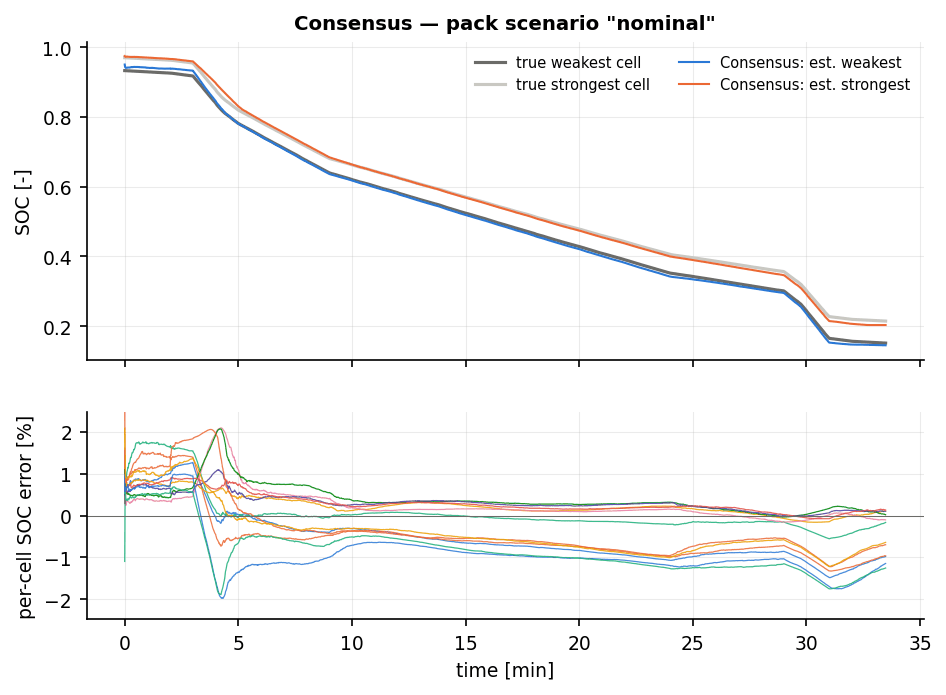
\includegraphics[width=\textwidth]{figures/pack_Consensus_nominal.png}
\caption{Consensus (ring, $\gamma=0.4$) on the nominal eVTOL mission: per-cell SOC with the
min/mean/max envelope (top), per-cell error (middle), current (bottom).}
\end{figure}
\begin{figure}[H]\centering
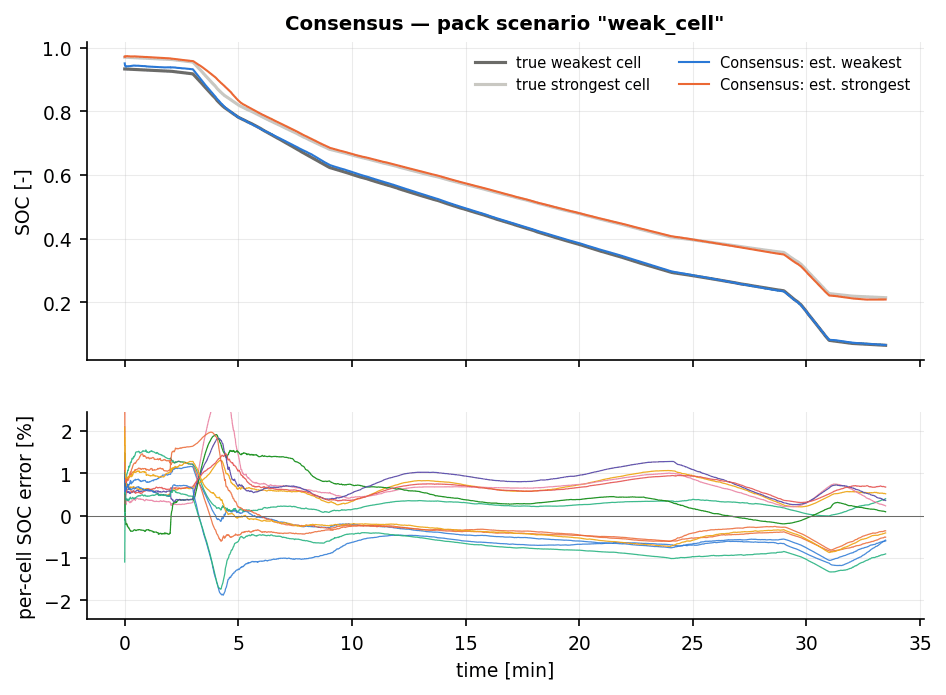
\includegraphics[width=\textwidth]{figures/pack_Consensus_weak_cell.png}
\caption{Consensus on \texttt{weak\_cell}: node 5 owns the aged cell and is the only node whose
measurement is atypical; its neighbours' information and the consensus term keep its common
estimate with the network while the delta filter absorbs the divergence.}
\end{figure}

\begin{center}\small
\begin{tabular}{@{}lcccc|cccc@{}}
\toprule
& \multicolumn{4}{c|}{\estname{Consensus}} & \multicolumn{4}{c}{\estname{Decentralized-EKF}} \\
Scenario & rmse & rmse$_{\min}$ & ss & max & rmse & rmse$_{\min}$ & ss & max \\
\midrule
\texttt{nominal}          & 0.0066 & 0.0056 & 0.0066 & 0.028 & 0.0123 & 0.0081 & 0.0134 & 0.046 \\
\texttt{init\_error}      & 0.0063 & 0.0050 & 0.0063 & 0.029 & 0.0118 & 0.0082 & 0.0129 & 0.042 \\
\texttt{current\_bias}    & 0.0079 & 0.0086 & 0.0052 & 0.036 & 0.0137 & 0.0088 & 0.0148 & 0.056 \\
\texttt{weak\_cell}       & 0.0064 & 0.0055 & 0.0059 & 0.028 & 0.0129 & 0.0129 & 0.0137 & 0.048 \\
\texttt{noise\_step}      & 0.0069 & 0.0057 & 0.0071 & 0.028 & 0.0122 & 0.0084 & 0.0131 & 0.045 \\
\texttt{large\_imbalance} & 0.0139 & 0.0203 & 0.0128 & 0.090 & 0.0174 & 0.0245 & 0.0179 & 0.061 \\
\midrule
\si{\nano\second}/step & \multicolumn{4}{c|}{6344 (529/node)} & \multicolumn{4}{c}{3860 (322/node)} \\
bytes & \multicolumn{4}{c|}{9224} & \multicolumn{4}{c}{52032} \\
messages/step & \multicolumn{4}{c|}{216} & \multicolumn{4}{c}{0} \\
\bottomrule
\end{tabular}
\end{center}
(Means over three seeds.)

\paragraph{Against the decentralised baseline.} The KCF halves the error of
\estname{Decentralized-EKF} in every scenario (\num{0.0066} versus \num{0.0123} on
\texttt{nominal}) with the same number of processors and one sixth of the memory, and it is the
best of the whole family on \texttt{max\_cell\_err} in four of six scenarios (\num{0.028} on
\texttt{nominal} against \num{0.031} for the centralised optimum), because each node keeps its own
common state and therefore absorbs its own cell's peculiarity instead of averaging it away.

\paragraph{The gap to the centralised optimum, and how the topology closes it.} Registered
estimators from the three-seed run, topology variants from the paired two-seed ablation run;
rmse:
\begin{center}\small
\begin{tabular}{@{}lccccr@{}}
\toprule
Variant & \texttt{nominal} & \texttt{weak\_cell} & \texttt{large\_imb.} & channels fused & \si{\nano\second}/step \\
\midrule
\estname{InfoFusion} (centralised)     & 0.0055 & 0.0057 & 0.0094 & 12 & 1463 \\
KCF, complete graph ($d=11$)           & 0.0046 & 0.0054 & 0.0071 & 12 & 6995 \\
KCF, ring ($d=2$, default)             & 0.0066 & 0.0064 & 0.0139 &  3 & 6344 \\
KCF, line ($d=2$, ends $d=1$)          & 0.0068 & 0.0065 & 0.0138 &  3 & 6411 \\
\bottomrule
\end{tabular}
\end{center}
The ring pays \SI{20}{\percent} on \texttt{nominal} and \SI{48}{\percent} on
\texttt{large\_imbalance} relative to the centralised optimum: exactly the deficit expected from
fusing \num{3} of \num{12} channels. Closing the graph removes the gap and in fact beats the
centralised filter slightly (\num{0.0046} against \num{0.0055}, and \num{0.0071} against
\num{0.0094} on \texttt{large\_imbalance}) --- with $d=N_c-1$ each node performs the full
centralised update \emph{and} keeps a private common state biased towards its own cell, which is a
better model of the true per-cell state than one shared common state plus a scalar deviation.
Closing a line into a ring costs one link and is worth a few percent.

\paragraph{The consensus gain behaves as Proposition~\ref{prop:con-stab} predicts.} Sweeping
$\gamma$ on the ring in one paired two-seed run (so the $\gamma=\num{0.4}$ column differs in the
last digit from the three-seed table above), rmse:
\begin{center}\small
\begin{tabular}{@{}lcccc@{}}
\toprule
$\gamma$ & 0 & 0.4 (default) & 2 & 8 \\
\midrule
\texttt{nominal}     & 0.0069 & 0.0070 & 0.0070 & 0.0101 \\
\texttt{init\_error} & 0.0067 & 0.0068 & 0.0068 & 0.0178 \\
\texttt{weak\_cell}  & 0.0066 & 0.0066 & 0.0066 & 0.0108 \\
\bottomrule
\end{tabular}
\end{center}
Between $\gamma=0$ and $\gamma=2$ the differences are below \SI{2}{\percent}, i.e.\ within the
seed-to-seed scatter --- the normalisation \eqref{eq:con-eps} keeps the effective gain
$\varepsilon\norm{\bm{M}_j}_F$ at \num{1.3e-4} in steady state, far inside the stability region,
so the consensus term is a gentle correction rather than a dominant one. At
$\gamma=8$ it becomes strong enough to over-smooth the node estimates and the error grows by
\SI{50}{\percent} --- degradation, not divergence, again as \eqref{eq:con-epsbound} predicts. The
small effect of $\gamma$ here is a property of this benchmark, not of the method: as
Remark~\ref{rem:con-purpose} explains, all twelve nodes see equally good measurements of the same
state, so there is little disagreement for consensus to remove. Its value would show in a
dropped-channel or cold-start-node scenario, which this benchmark does not contain.

\paragraph{The nodes do not, and should not, agree exactly.} The spread
$\max_j\hat{\bar\soc}_j - \min_j\hat{\bar\soc}_j$ of the twelve nodes' common estimates measured
on the nominal mission is \num{0.024} at $k=0$, \num{0.013} after \SI{100}{\second} and
\num{0.033} at the end of the flight --- it shrinks during the initial transient but never goes
to zero. This is not a failure of Assumption~\ref{as:con-conn}: with $\varepsilon\norm{\bm{M}_j}
\sim\num{1e-4}$ the consensus term is far weaker than each node's own measurement, so node $j$'s
``common'' estimate settles close to \emph{its own} cell's SOC rather than to the module mean. That
is exactly why the KCF has the lowest \texttt{max\_cell\_err} of the family: the per-cell estimate
$\hat{\bar\soc}_j+\Delta\hat\soc_j$ is then largely a private, reduced-order per-cell filter, with
the neighbourhood information acting as a stabiliser. Raising $\gamma$ to force true consensus
(the $\gamma=8$ column) makes the nodes agree more and the per-cell estimates worse.

\paragraph{Deviation compensation matters more here than anywhere else.} Turning it off costs
\num{0.0082} instead of \num{0.0066} on \texttt{nominal} and \num{0.0123} instead of \num{0.0064}
on \texttt{weak\_cell} --- twice the penalty seen by the centralised filter. The reason is
structural: a centralised or federated fusion averages the $N_c$ deviations away
($\sum_j\delta_j\approx0$), but a node with two neighbours averages only three of them, so the
uncompensated deviation survives in its common estimate.

\paragraph{Where it is weakest.} \texttt{large\_imbalance}, for the same reason: with a
\SI{5}{\percent} spread the neighbourhood average of the deviations is far from zero, and the
node's common estimate inherits it (rmse \num{0.0139} against \num{0.0094} centralised). This is
the intrinsic limitation of local fusion and is the price of having no master.

\section{Summary}
Use the Kalman-consensus filter when the pack must keep working with no central node and the
physical topology is a chain or a ring --- the message size is independent of $N_c$, every node
produces a usable SOC on its own, and losing a node leaves a connected graph. Keep the
covariance-normalised gain \eqref{eq:con-eps}; it makes $\gamma$ a non-critical tuning parameter
(anything in $[0,2]$ behaves identically here) and guarantees stability across the whole range of
filter confidence. Expect to pay \SIrange{20}{50}{\percent} more error than the centralised
optimum on a degree-2 graph, recoverable by adding links, and compensate the per-cell deviation
before the local update --- without it, local fusion has too few channels to average the
deviations away. Do not use it when a master already exists and is trusted: Chapters
\ref{ch:infofusion} and \ref{ch:federated} then give a better estimate for less arithmetic.
